\section{Інтерпретація результатів моделювання}

\subsection{Інтерпретація результатів}

Двох смуг аеропорту недостатньо. Щоб посадити 10~літаків за годину, кожен з яких займає смугу на 35~хвилин, потрібно в середньому 5,83~смуги, а їх лише дві. Тому черга росте, доки її не обмежує відліт літаків через 140~хвилин. У такому режимі майже кожен літак чекає довше за поріг дозаправки, тож аеропорт платить за дозаправку кожного, а дохід отримує лише за третину з них. Витрати на дозаправку (близько 1000~грн) переважують дохід від посадки з очікуванням (близько 1500~грн), помножений на частку тих, хто сів. Звідси збиток 42,5~млн~грн на рік.

Третя, четверта і п'ята смуги збільшують прибуток на 22--26~млн~грн кожна: кожна приймає ще близько 15\,000~літаків на рік, але смуги все ще перевантажені, і майже всі літаки дозаправляються. Перелом настає між п'ятою і сьомою смугами, коли пропускна здатність смуг перевищує потік літаків: черга зникає, дозаправки й відльоти припиняються, і прибуток стрибає з 28,6 до 151,2~млн~грн на рік. Після семи смуг прибуток зростає ледь помітно, бо майже всі літаки й так сідають і зростає лише частка посадок без очікування (2000~грн замість 1500).

Тому час окупності має чіткий мінімум на семи смугах. Будівництво п'яти додаткових смуг коштує 15~млн~грн і дає приріст прибутку 193,7~млн~грн на рік, тобто окупається за 0,93~місяця, або близько 28~діб. Шоста смуга окупилась би за 0,96~місяця, восьма -- за 1,06~місяця. Ці різниці невеликі в абсолютних числах, але довірчі інтервали не перетинаються, тож сім смуг -- справді найкращий варіант за умовами завдання.

\subsection{Пропозиції щодо поліпшення функціонування системи}

На основі результатів моделювання пропонується збудувати п'ять додаткових посадкових смуг, довівши їх кількість до семи. Очікуване поліпшення порівняно з поточним станом за результатами експериментів (таблиця~\ref{tab:payback}):
\begin{itemize}
\item річний прибуток зростає з $-42{,}5$ до 151,2~млн~грн;
\item кількість літаків, що відлітають в інші аеропорти, зменшується з 57\,511 на рік до нуля;
\item кількість дозаправок зменшується з 87\,544 до 479 на рік;
\item середнє очікування посадки скорочується з 132,1 до 8,8~хв.
\end{itemize}

Інтенсивність потоку літаків у реальному аеропорту змінюється з часом, тому важливо, чи лишиться рекомендація правильною, якщо потік буде іншим. Для перевірки зроблено пробний запуск моделі за інтенсивності 8 і 12~літаків за годину, тобто на 20~\% менше і більше за задану, з тими самими умовами експерименту: 51~прогін по 365~діб для кожної кількості смуг. Результати наведено в таблиці~\ref{tab:sensitivity} і на рисунку~\ref{fig:sensitivity}.

\begingroup
\fontsize{12}{14}\selectfont
\begin{kpitable}{|L{1.0cm}|L{2.3cm}|L{2.0cm}|L{2.3cm}|L{2.0cm}|L{2.3cm}|L{2.0cm}|}{Прибуток і час окупності за різної інтенсивності надходження літаків\label{tab:sensitivity}}{\multirow{2}{*}{\textbf{$n$}} & \multicolumn{2}{c|}{\textbf{8 літаків / год}} & \multicolumn{2}{c|}{\textbf{10 літаків / год}} & \multicolumn{2}{c|}{\textbf{12 літаків / год}} \\ \cline{2-7}
 & \textbf{$P$, млн грн/рік} & \textbf{$T_{\Delta}$, міс.} & \textbf{$P$, млн грн/рік} & \textbf{$T_{\Delta}$, міс.} & \textbf{$P$, млн грн/рік} & \textbf{$T_{\Delta}$, міс.}}
2 & \textminus{}25,0 & -- & \textminus{}42,5 & -- & \textminus{}60,0 & -- \\ \hline
3 & \textminus{}2,2 & 1,584 & \textminus{}20,0 & 1,601 & \textminus{}37,6 & 1,603 \\ \hline
4 & 25,0 & 1,442 & 2,6 & 1,596 & \textminus{}15,0 & 1,597 \\ \hline
5 & 98,3 & 0,876 & 28,6 & 1,519 & 7,6 & 1,596 \\ \hline
6 & 124,2 & 0,965 & 107,7 & 0,959 & 32,5 & 1,556 \\ \hline
7 & 132,0 & 1,146 & 151,2 & 0,929 & 107,9 & 1,072 \\ \hline
8 & 136,2 & 1,340 & 162,2 & 1,055 & 176,8 & 0,912 \\ \hline
9 & 138,4 & 1,543 & 168,3 & 1,196 & 191,2 & 1,003 \\ \hline
10 & 139,4 & 1,752 & 171,7 & 1,345 & 199,6 & 1,109 \\ \hline
11 & 139,9 & 1,965 & 173,5 & 1,500 & 204,4 & 1,225 \\ \hline
12 & 140,1 & 2,181 & 174,5 & 1,659 & 207,2 & 1,347 \\ \hline

\end{kpitable}
\endgroup

\begin{figure}[H]
\centering
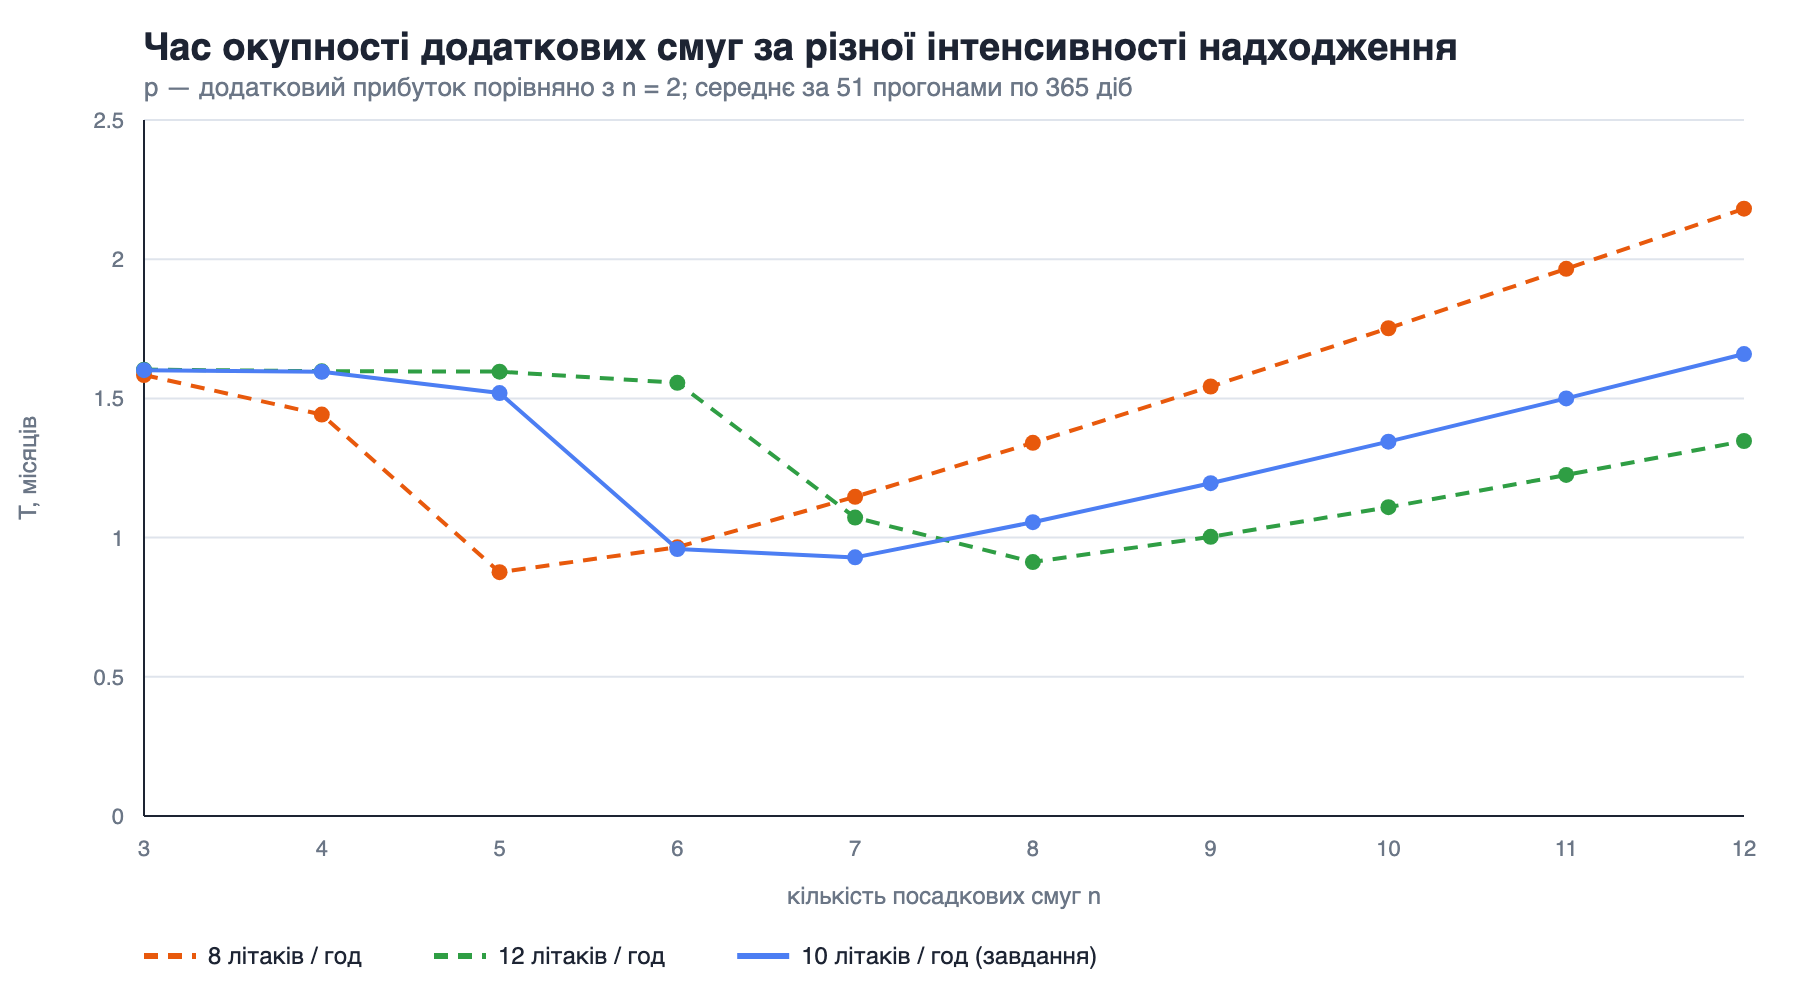
\includegraphics[width=0.92\textwidth]{sensitivity.png}
\caption{Час окупності додаткових смуг за різної інтенсивності надходження літаків}
\label{fig:sensitivity}
\end{figure}

Оптимальна кількість смуг залежить від потоку. За 8~літаків на годину найкраще мати 5~смуг ($T_{\Delta} = 0{,}876$~міс.), за 12~літаків -- 8~смуг ($T_{\Delta} = 0{,}912$~міс.). Закономірність та сама, що й для заданого потоку: потрібне середнє навантаження становить $\lambda \cdot t_s$, тобто 4,67, 5,83 і 7,0~смуги, і оптимум -- найменша кількість смуг, що з запасом перевищує це навантаження. Кількість смуг, рівна навантаженню з запасом менше 0,2~смуги (6~смуг за 10~літаків на годину), гірша: черга ще накопичується в години піків, і частина літаків дозаправляється.

Рекомендація чутлива до похибок у потоці, але помилка в бік більшої кількості смуг коштує мало. Якщо збудувати 5~додаткових смуг, а потік виявиться 12~літаків на годину, окупність становитиме 1,07~міс. замість найкращих 0,91. Якщо ж збудувати 6~додаткових смуг за заданого потоку, окупність становитиме 1,06~міс. замість 0,93. Натомість нестача смуг обходиться дорого: за 12~літаків на годину і 6~смугах прибуток лише 32,5~млн~грн на рік проти 107,9 за 7~смуг.

Отже, за заданої інтенсивності 10~літаків на годину слід будувати 5~додаткових смуг. Якщо аеропорт очікує зростання потоку, доцільно передбачити місце для шостої додаткової смуги й збудувати її, коли інтенсивність наблизиться до 12~літаків на годину.

\subsection{Висновки до розділу}

Двох смуг недостатньо для потоку 10~літаків на годину, тому аеропорт збитковий через масові дозаправки й відльоти. Найкоротша окупність, 0,93~міс., досягається за п'яти додаткових смуг, що й пропонується збудувати: це дає прибуток 151,2~млн~грн на рік, усуває відльоти і скорочує очікування до 8,8~хв. Пробний запуск за 8 і 12~літаків на годину показав, що оптимальна кількість смуг -- найменша, яка з запасом перевищує середнє навантаження $\lambda \cdot t_s$, і що за зростання потоку до 12~літаків на годину варто додати шосту смугу.
